% SPDX-FileCopyrightText: 2024 Lukas Zirpel <thesis+lukas@zirpel.de>
% SPDX-License-Identifier: GPL-3.0-only

\documentclass[a4paper,11pt, openany, draft]{book} %Remove draft option to hide ToDos

% SPDX-FileCopyrightText: 2024 Lukas Zirpel <thesis+lukas@zirpel.de>
% SPDX-License-Identifier: GPL-3.0-only

\makeatletter

% Packages needed
\usepackage{geometry}
\usepackage[small,compact]{titlesec}
\usepackage[final]{listings}
\usepackage{amsmath}
\usepackage{amssymb}
\usepackage{tipa}
\usepackage[english]{babel}
\usepackage{lstautogobble}
\usepackage{proof}
\usepackage{bussproofs}
\usepackage{xparse}
\usepackage{needspace}
\usepackage{xspace}
\usepackage{mathpartir}
\usepackage{tikz}
\usetikzlibrary{arrows}
\usetikzlibrary{fit}
\usetikzlibrary{positioning}
\usepackage[amsmath,hyperref,thmmarks]{ntheorem}
\usepackage{parskip}
\usepackage{scrextend}
\usepackage{wrapfig}
\usepackage[nottoc]{tocbibind}
\usepackage{caption}
\usepackage{coqtheorem}
\usepackage[nameinlink]{cleveref}


% For the font
\usepackage{fontspec}
\usepackage{tgpagella}
\usepackage[euler-digits,small]{eulervm}
\linespread{1.025}              % Palatino leads a little more leading

\usepackage{fancyhdr}
\usepackage[obeyDraft]{todonotes}
\setlength{\marginparwidth}{3cm}

\usepackage[toc]{glossaries}
\usepackage[backend=biber,style=numeric,datamodel=archiving]{biblatex}

% SPDX-FileCopyrightText: 2024 Lukas Zirpel <thesis+lukas@zirpel.de>
% SPDX-License-Identifier: GPL-3.0-only

%% Macros
\newcommand{\M}[1]{\ensuremath{\textit{#1}}} % \mathup
\newcommand{\imp}{\mathbin{\rightarrow}~}
\newcommand{\Imp}{\mathbin{\Rightarrow}~}
\renewcommand{\iff}{\mathbin{\leftrightarrow}}
\newcommand{\defeq}{\mathrel{\mathop:=}}

\newcommand{\dd}[2]{\ensuremath{#1_1,\dots,#1_{#2}}}  % x_1,...,x_n
\newcommand{\ddd}[2]{\ensuremath{#1_1\dots\,#1_{#2}}}  % x_1...x_n
\newcommand{\col}{\colon}
\newcommand{\set}[1]{\ensuremath{\{#1\}}}
\newcommand{\mset}[2]{\set{\,#1\mid#2\,}}
\newcommand{\eset}{\ensuremath{\emptyset}}
\newcommand{\incl}{\ensuremath{\subseteq}}
\newcommand{\bnfor}{~|~} %|
\newcommand{\qedsq}{\hfill\ensuremath{_\blacksquare}}

\newcommand{\blankpage}{\newpage
\thispagestyle{empty}
\mbox{}
\newpage}

\renewcommand\qed {{% set up
\parfillskip=0pt % so \par doesnt push \square to left
\widowpenalty=10000 % so we dont break the page before \square
\displaywidowpenalty=10000 % ditto
\finalhyphendemerits=0 % TeXbook exercise 14.32
%
% horizontal
\leavevmode % \nobreak means lines not pages
\unskip % remove previous space or glue
\nobreak % don't break lines
\hfil % ragged right if we spill over
\penalty50 % discouragement to do so
\hskip.2em % ensure some space
\null % anchor following \hfill
\hfill % push \square to right
$\square$% % the end-of-proof mark
%
% vertical
\par}} % build paragraph


% SPDX-FileCopyrightText: 2024 Lukas Zirpel <thesis+lukas@zirpel.de>
% SPDX-License-Identifier: GPL-3.0-only

\newlength{\blockindent}
\setlength{\blockindent}{8mm}

\theoremstyle{coqtheorem}

\newtheorem{lemma}{Lemma}[chapter]
\newtheorem{proposition}[lemma]{Proposition}
\newtheorem{fact}[lemma]{Fact}
\newtheorem{theorem}[lemma]{Theorem} %Uncomment this line if you want to use usual theorems from ntheorem
\newtheorem{corollary}[lemma]{Corollary}
\newtheorem{definition}[lemma]{Definition}
\newtheorem{exercise}[lemma]{Exercise}

%% Beweise
\theoremstyle{nonumberplain}
\theorembodyfont{\normalfont}
\theoremsymbol{\qed}
\newtheorem{proof}{Proof}
\providecommand*{\toclevel@proof}{0}
\theoremclass{LaTeX}


% From https://tex.stackexchange.com/questions/302968/biblatex-add-a-second-url-where-content-is-archived
\NewBibliographyString{archivedat,archivedon}
\DefineBibliographyStrings{english}{%
  archivedat = {archived at},
  archivedon = {on},
}

\DeclareFieldFormat{archiveurl}{\bibstring{archivedat}\space\url{#1}}
\DeclareFieldFormat{archivedate}{\bibstring{archivedon}\space#1}

\newbibmacro*{archiveurl}{\printfield{archiveurl}}
\newbibmacro*{archivedate}{\printarchivedate}

\renewbibmacro*{url+urldate}{%
  \usebibmacro{url}%
  \iffieldundef{urlyear}
    {}
    {\setunit*{\addspace}%
     \usebibmacro{urldate}}%
  \setunit{\addcomma\space}%
  \usebibmacro{archiveurl}%
  \iffieldundef{archiveyear}
    {}
    {\setunit*{\addspace}%
     \usebibmacro{archivedate}}}


\addbibresource{bibliography.bib}

%% Geometrie
\newdimen\lines
\setbox\@tempboxa\hbox{(Programmierung)}
\lines=\ht\@tempboxa
\advance\lines by\dp\@tempboxa

\newlength{\exb}
\settowidth{\exb}{\normalfont x}
\geometry{%
  a4paper,%
  includehead,% (=> head is part of total body)
  ignorefoot,% (=> foot is not part of total body)
  top=3cm,% (top of paper |---| top of total body)
  totalwidth=70\exb,% (width of total body)
  totalheight=215mm,% (height of total body)
  headheight=1\lines,%
  headsep=2.5\lines,%
  foot=4\lines,% (bottom of text body |---| _bottom_ of foot)
  hcentering%
}%

\newcommand{\setauthor}[1]{\author{#1}\def\theauthor{#1}}
\newcommand{\settitle}[1]{\title{#1}\def\thetitle{#1}}

\newcommand{\advisor}[1]{\def\theadvisor{#1}}
\newcommand{\reviewerOne}[1]{\def\thereviewerOne{#1}}
\newcommand{\reviewerTwo}[1]{\def\thereviewerTwo{#1}}
\newcommand{\university}[1]{\def\theuniversity{#1}}
\newcommand{\faculty}[1]{\def\thefaculty{#1}}
\newcommand{\thesistype}[1]{\def\thethesistype{#1}}
\newcommand{\subdate}[3]{\def\thesubday{#1} \def\thesubmonth{#2} \def\thesubyear{#3} }
\newcommand{\city}[1]{\def\thecity{#1}}

\newcommand{\maketitlepage}{
  \begin{titlepage}
    \begin{center}
      \newcommand{\HRule}{\rule{\linewidth}{0.5mm}}
      \begin{minipage}{0.2\textwidth}
        
\includegraphics[draft=false,width=0.9\textwidth]{logo.eps}
      \end{minipage}
      \begin{minipage}{0.7\textwidth}
        \centering \textsc{{\Huge \theuniversity}}

        \centering \textsc{\footnotesize \thefaculty}
      \end{minipage}
      \vspace{1cm}

      \textsc{\thethesistype ~Thesis}\\[0.3cm]
      % Title
      \HRule \\[0.4cm]
      { \Huge \scshape \thetitle \\[0.4cm] }

      \HRule \\[1.5cm]

      % Author and supervisor
      \noindent
      \begin{minipage}{0.4\textwidth}
        \begin{flushleft} \Large
          \emph{Author}\\
          \theauthor
        \end{flushleft}
      \end{minipage}%
      \begin{minipage}{0.4\textwidth}
        \begin{flushright} \Large
          \emph{Advisor} \\
          \theadvisor

        \end{flushright}
      \end{minipage}

      \noindent
      \begin{minipage}{1\textwidth}
        \vspace{7cm}
        \begin{center} \large
          \emph{Reviewers} \\
          \thereviewerOne\\
          \thereviewerTwo
        \end{center}
      \end{minipage}

      \vfill

      {\large Submitted: \thesubday\textsuperscript{th} \thesubmonth~\thesubyear}

    \end{center}
  \end{titlepage}
}

\newcommand{\statementpage}{
~ \vspace*{2cm} ~

\textbf{Eidesstattliche Erklärung}

Ich erkläre hiermit an Eides statt, dass ich die vorliegende Arbeit
selbstständig verfasst und keine anderen als die angegebenen Quellen und
Hilfsmittel verwendet habe.

\textbf{Statement in Lieu of an Oath}

I hereby confirm that I have written this thesis on my own and that I
have not used any other media or materials than the ones referred to in
this thesis.


~ \vspace{3cm} ~

\textbf{Einverständniserklärung}

Ich bin damit einverstanden, dass meine (bestandene) Arbeit in beiden
Versionen in die Bibliothek der Informatik aufgenommen und damit
veröffentlicht wird.
% \begin{center}
% \Large

\textbf{Declaration of Consent}

I agree to make both versions of my thesis (with a passing grade)
accessible to the public by having them added to the library of the
Computer Science Department.

\vspace*{3cm}

\thecity, \thesubday$^{\text{th}}$ \thesubmonth, \thesubyear

\newpage
}

\makeatother

%%% Local Variables:
%%% mode: latex
%%% TeX-master: "thesis"
%%% End:

\tolerance=200

\settitle{Measuring the overhead of encryption and censorship evasion protocols over lossy links}
\setauthor{Lukas Zirpel}
\advisor{Dr.-Ing Tobias Fiebig}
\reviewerOne{Prof. Anja Feldmann, Ph.D.}
\reviewerTwo{TODO}
\university{Saarland University}
\faculty{Faculty of Mathematics and Computer Science}
\thesistype{Bachelor's}
\subdate{20}{February}{2025}
\city{Saarbrücken}
\setBaseUrl{{https://www. ... .de/coq/}}

\DeclareTextFontCommand{\emph}{\bfseries}


\pagenumbering{roman}

\setlength{\headheight}{15pt}

\pagestyle{fancy}
\renewcommand{\chaptermark}[1]{ \markboth{#1}{} }
%\renewcommand{\sectionmark}[1]{ \markright{#1}{} }

\fancyhf{}
\fancyhead[LE,RO]{\thepage}
\fancyhead[RE]{\textit{ \nouppercase{\leftmark}} }
\fancyhead[LO]{\textit{ \nouppercase{\rightmark}} }

\fancypagestyle{plain}{
	\fancyhf{}
	\renewcommand{\headrulewidth}{0pt}
	\renewcommand{\footrulewidth}{0pt}
}

\begin{document}

\thispagestyle{empty}

\maketitlepage

\statementpage

\chapter*{Abstract}
\addcontentsline{toc}{chapter}{\numberline{}Abstract}
% SPDX-FileCopyrightText: 2024 Lukas Zirpel <thesis+lukas@zirpel.de>
% SPDX-License-Identifier: GPL-3.0-only

Censorship evasion tools are crucial for maintaining access to information in censored environments.
This thesis evaluates the overhead of several popular censorship circumvention protocols under realistic network conditions, examining their impact on key network metrics relevant to their practical deployment and effectiveness.
We employ a rigorous methodology, combining virtualized prototyping with real-world hardware testing.
Our setup allows for experiments in reproducible environments and controlled network impairment simulation.
Our experiments analyze the behavior of WireGuard, DNS tunneling (iodine), ICMP tunneling (ICMPTX), and Tor pluggable transports (obfs4, Snowflake) under controlled network impairments, varying parameters such as packet loss, latency, jitter, and MTU.
We present results on packet overhead, throughput, and resource utilization (CPU and RAM consumption), revealing the performance trade-offs inherent in each protocol.
We also investigate the impact of these protocols on the Maximum Transmission Unit (MTU) and discuss its implications for network performance.
Despite encountering implementation challenges with ICMPTX and iodine, our rigorous methodology, combining virtualized and real-world testing, allows for a detailed analysis of several key censorship circumvention protocols.
Future work will build upon this foundation, addressing the limitations encountered and expanding the scope of protocol evaluation.

\keywords{Censorship Evasion, Network Impairments, Network Performance, Protocol Overhead, Throughput, Latency}


%%% Local Variables:
%%% TeX-master: "thesis"
%%% End:


\newpage

\chapter*{Acknowledgements}
% SPDX-FileCopyrightText: 2024 Lukas Zirpel <thesis+lukas@zirpel.de>
% SPDX-License-Identifier: GPL-3.0-only

I thank all my friends. \todo{Find friends.}

%%% Local Variables:
%%% TeX-master: "thesis"
%%% End:



\addtocontents{toc}{\vspace{5mm}}

\tableofcontents

\listoftodos

\clearpage
\pagenumbering{arabic}

% SPDX-FileCopyrightText: 2024 Lukas Zirpel <thesis+lukas@zirpel.de>
% SPDX-License-Identifier: GPL-3.0-only

\chapter{Introduction}


Many places in the world encounter internet censorship.
To try to get around the censorship, numerous different techniques, some very creative, were developed.
They obfuscate data and either hide it from or make it seem like innocent data to the censors \todo{mention steganography?}.

\begin{itemize}
  \item Zensur sieht in der Realität anders aus
\end{itemize}
Running these protocols on phones or other mobile devices also constrains the available CPU and RAM resources.

However, these censorship circumvention protocols are likely developed in laboratory conditions with ideal networks and plentiful computational resources.
These are not the same conditions encountered in the real world, where networks may have a high latency, high packet loss and low throughput.

For this reason, we aim to analyze the behaviour of different censorship circumvention protocols under these conditions.
Specifically, we ask the research question:
\emph{``Haupt-research question here.''}
This research question breaks up into the following sub-questions:
\begin{itemize}
  \item ...
  \item ...
  \item ...
  \item ...
\end{itemize}

We answer these research questions using a simulation environment.
Accurately simulating real-world conditions is challenging.
We use \href{https://man7.org/linux/man-pages/man8/tc-netem.8.html}{netem}, Linux's network emulator as a reasonable approximation of the real world.

In order to evaluate different protocols with many different network conditions, we need an automated testing setup.
We will first use the NixOS testing framework to simulate our test setup using VMs for experimentation and then run the setup on real hardware to make sure that our results are not influenced by virtualisation.
Censorship circumvention protocols usually work like a network tunnel and transport the actual payload inside of them.

We will analyze the latency and packet size each protocol adds.
We are also looking for pathological behaviour of the protocols such as unreasonable packet loss or latencies inside the tunnel compared to outside under unfavorable network conditions.
We will also analyze the CPU and RAM resources each protocol consumes.

\noindent\textbf{Structure:}
The remainder of this thesis is structured as follows:
% Background
In Section~\ref{TODO} we will ...
% Methodik
Subsequently, in Section~\ref{TODO} we (present tense) ...

\todo{chapter instead of section}

% SPDX-FileCopyrightText: 2024 Lukas Zirpel <thesis+lukas@zirpel.de>
% SPDX-License-Identifier: GPL-3.0-only

\chapter{Background and Related Work}

\todo{There must be some analysis on WireGuard}
\todo{Split related work into separate chapter?}

There are a number of \href{https://brianlinkletter.com/2023/02/network-emulators-and-network-simulators-2023/}{existing network simulators} for simulating complex network setups with routers, switches, etc..
Many of them focus on simulating mesh networks for testing routing protocols, see for example \href{https://github.com/mwarning/meshnet-lab}{Mesh Network Lab}.
Our network is very simple, while the complexity lies in the configuration of the hosts.
This is why we chose the NixOS testing framework.
It allows declararing the exact configuration of the hosts and the virtual network in code.
All dependencies are pinned in a lock file and no outside dependencies are used so everything should still be reproducible in a decade or more without having to e.g. hunt for ancient Ubuntu images.

\section{Network data transmission and MTU}

\section{Censorship}
\subsection{Preventing content access}
\subsection{Censorship evasion}

\section{Network Throughput Performance Measurements}

\section{Reproducibility in Network Measurement}


% SPDX-FileCopyrightText: 2024 Lukas Zirpel <thesis+lukas@zirpel.de>
% SPDX-License-Identifier: GPL-3.0-only

\chapter{Methodology}
\label{chap:methodology}

\section{Experimental design}
\begin{itemize}
  \item Was haben wir vor?
  \item Wie können wir das erreichen?
  \item Was müssen wir dabei beachten?
\end{itemize}

\section{Testbed}
\begin{itemize}
  \item Was haben wir zusammengesteckt (Figure)
  \item Warum Hardware und nicht virtuell?
  \item Warum Nix?
\end{itemize}

\section{Scenario Selection}
\subsection{Protocols to test}
\begin{itemize}
  \item none, as a baseline
  \item WireGuard
  \item DNS tunnel (iodine)
  \item ICMP tunnel (ICMPTX)
  \item phantun
  \item Various Tor Protocols
\end{itemize}

\todo{provide reasoning why we chose these protocols specifically and describe them briefly}

\subsection{Parameters to test}
\begin{itemize}
  \item Packet loss
  \item Latency
  \item Reorder packets
  \item Duplicate packets
  \item MTU
\end{itemize}
explain why these parameters, etwas wie Tabelle, Spalten Parameter







In an attempt to save space...
The \href{https://en.wikipedia.org/wiki/Pcap}{.pcap} files only compress well if the data is not encrypted or otherwise scrambled.
The files could either be explicitly compressed with a compression tool like zstd or the compression could be done at the filesystem level, e.g. with \href{https://openzfs.org/wiki/Main_Page}{ZFS}.


Since we're only interested in measuring what happens during the actual test and not in the connection setup and teardown of iperf3, we use heuristics
The connection setup and teardown of iperf3 should not be part of the analysis, hence a heuristic is employed to ignore this part of the packet capture. To find the start of the test, we find the first packet which is larger than a threshhold. To find the end of the test, we find the last packet which is larger than a threshhold and also ignore all packets that are sent after the duration of the test is over.

\href{https://en.wikipedia.org/wiki/Maximum_transmission_unit}{MTU}:
When the MTU inside of a tunnel is so large, that the overhead of the tunnel protocol would make the packet too big to be transported over the internet
Needs to be dealt with in some way. Usually by either dropping the packet and/or communicating the error to the application (\href{https://en.wikipedia.org/wiki/Path_MTU_Discovery}{Path MTU discovery}) or by fragmenting the packet. Since fragmentation has a relatively large performance overhead, this is usually avoided in practice. For this reason, we avoid fragmentation in this research by carefully choosing the MTU inside of the tunnels.

\todo{go through presentation and extract the info here}

\href{https://github.com/nix-community/nixos-anywhere}{nixos-anywhere} is used to quickly and reproducibly install the operating system on all machines.
nixos-anywhere uses \href{https://github.com/nix-community/disko}{disko} to partition and format the disks.


\todo{Define pre and post to mean before and after the router}

Data analysis pipeline:
\begin{itemize}
  \item run the experiment setup
  \item capture packets before and after the router and store them in .pcap files
  \item for each packet, extract the timestamp and compute the size and \href{https://en.wikipedia.org/wiki/BLAKE_(hash_function)#BLAKE3}{BLAKE3} hash of the IP payload and write the information into a \href{https://en.wikipedia.org/wiki/JSON}{JSON} file (done in analysis/parse/parse.py)
  \item for each packet captured before the router, find the same packet after the router (done in analysis/statistics/statistics.py). If we assume, that all packets are unique and that the router does not modify packets, then we can match up the unique hash of each packet before the router to some number of packets after the router. If no matching packet can be found after flowing through the router, it means that the packet was dropped. If more than one packet matches, it means that it was duplicated. If exactly one packet matches, it was routed without duplication or being dropped. For meaningful statistics, we group the data into short chunks (buckets) (1s) and compute bandwidth and packet counts over that bucket. The latency introduced by the router can be measured by computing the difference between the timestamps of each packet before the router and the first corresponding packet after the router. Dropped packets are ignored and for duplicated packets only the first arriving packet is counted. Throughput can be measured by summing up the IP payload \todo{should we measure at a different layer?} and dividing it by the time duration of the bucket. Dropped packets are ignored and packets which were duplicated count only once. The timestamp, dropped, duplicated and normal packet counts, throughput and a list of the latency of each packet are stored per bucket and written to a JSON file.
  \item Graphs are drawn using \href{https://matplotlib.org/}{Matplotlib} (done in analysis/graph/graph.py)
  \item \todo{for gaining insights, for example while comparing two different scenarios, it's helpful to plot data from multiple experiments in one plot. This still needs to be implemented.}
\end{itemize}


\todo{explain why we're capturing packets on a separate host.}
In the VM test setup, the virtual switch is configured to behave like a \href{https://en.wikipedia.org/wiki/Ethernet_hub}{hub} (\href{https://github.com/NixOS/nixpkgs/blob/0634959ae9c75ac8cab28dfcc9a0f045cf30dfc6/nixos/lib/test-driver/test_driver/vlan.py#L43}{\todo{reference to this}}), which makes it easy to capture the packets on both VLANs. On real hardware with a real switch, this is not quite as trivial. To replicate this setup with real hardware, we use Cisco's Switched Port Analyzer (SPAN), also known as port mirroring. Since enabling SPAN disables our ability to transmit packets from that interface for management purposes, we use a USB to Ethernet adapter for the management interface.
\todo{Specify the exact hardware model of the PCs and the SBCs}

% SPDX-FileCopyrightText: 2024 Lukas Zirpel <thesis+lukas@zirpel.de>
% SPDX-License-Identifier: GPL-3.0-only

\chapter{Results}
\label{chap:results}
\todo{beschreiben, was man sieht, Messungen irgendwie anordnen, innerhalb Sektion mit anderem vergleichen, z.B. MTU. zuerst nach Protokollen, dann Parameter}

In this section, we describe the results obtained by performing our
experiments.

\todo[inline]{Move the following into the Discussuion section}
\section{RQ1: How much packet size overhead does each protocol add?}
While we aimed to quantify the precise packet size overhead introduced by each protocol, our experimental setup did not allow for direct measurement of this metric.
However, it is important to note that the packet size overheads of many protocols are generally constant.
This overhead is due to the protocol's header, which is added to the data payload.
\todo[inline]{break down overhead of WireGuard and ICMPTX}

\section{RQ2: How much does the MTU decrease by using each protocol?}
For protocols that do not support fragmentation by themselves, the MTU decrease is directly related to the protocol's overhead.

\section{RQ3: How much additional latency does each protocol add?}
Unfortunately, the measurement setup was not designed correctly to accurately capture the additional latency introduced by each protocol.
Measuring additional latency introduced by a protocol requires observing the packets before they enter the tunnel and after they exit it.
The additional latency introduced by the protocol can then be analyzed by measuring how long each packet takes on average and subtracting the latency when no protocol is being used.
See \cref{fig:optimal_network_schematic} for a setup, which would be up to the task.
While we acknowledge the importance of latency as a performance metric, we are unable to reliably quantify it within the constraints of our current experimental design.

\section{RQ4: Do any protocols introduce additional packet loss?}
Similarly to latency measurements, our setup was not equipped to reliably measure packet loss introduced by the protocols themselves.



\section{RQ5: How much processing power and RAM does each protocol consume/require?}
did not measure

for userspace tunnel programs, can be measured using systemctl status

We are not aware of a good method of measuring the RAM usage of WireGuard.

We determine the CPU usage of WireGuard by looking at the output of \texttt{...} during a measurement.

The CPU usage is fairly constant over time and on both sides of the tunnel.

WireGuard used approximately \% of one CPU core



graphen beschreiben (Welche Achsen gibt es, etc.)
was sieht man?
warum sieht man das was man sieht?


graphs:
latency
packet counts
throughput

single or multi

single: axes:

for looking at a specific measurement in detail:

gives an overview of how consistent the measurement is

latency: box plot for every bucket: time, latency

packet counts: line with dot every bucket: time, counts

throughput: line with dot every bucket: time, throughput


to be able to see the influence of a parameter, multiple measurements in one graph:

\begin{figure}[tbh]
	\centering
	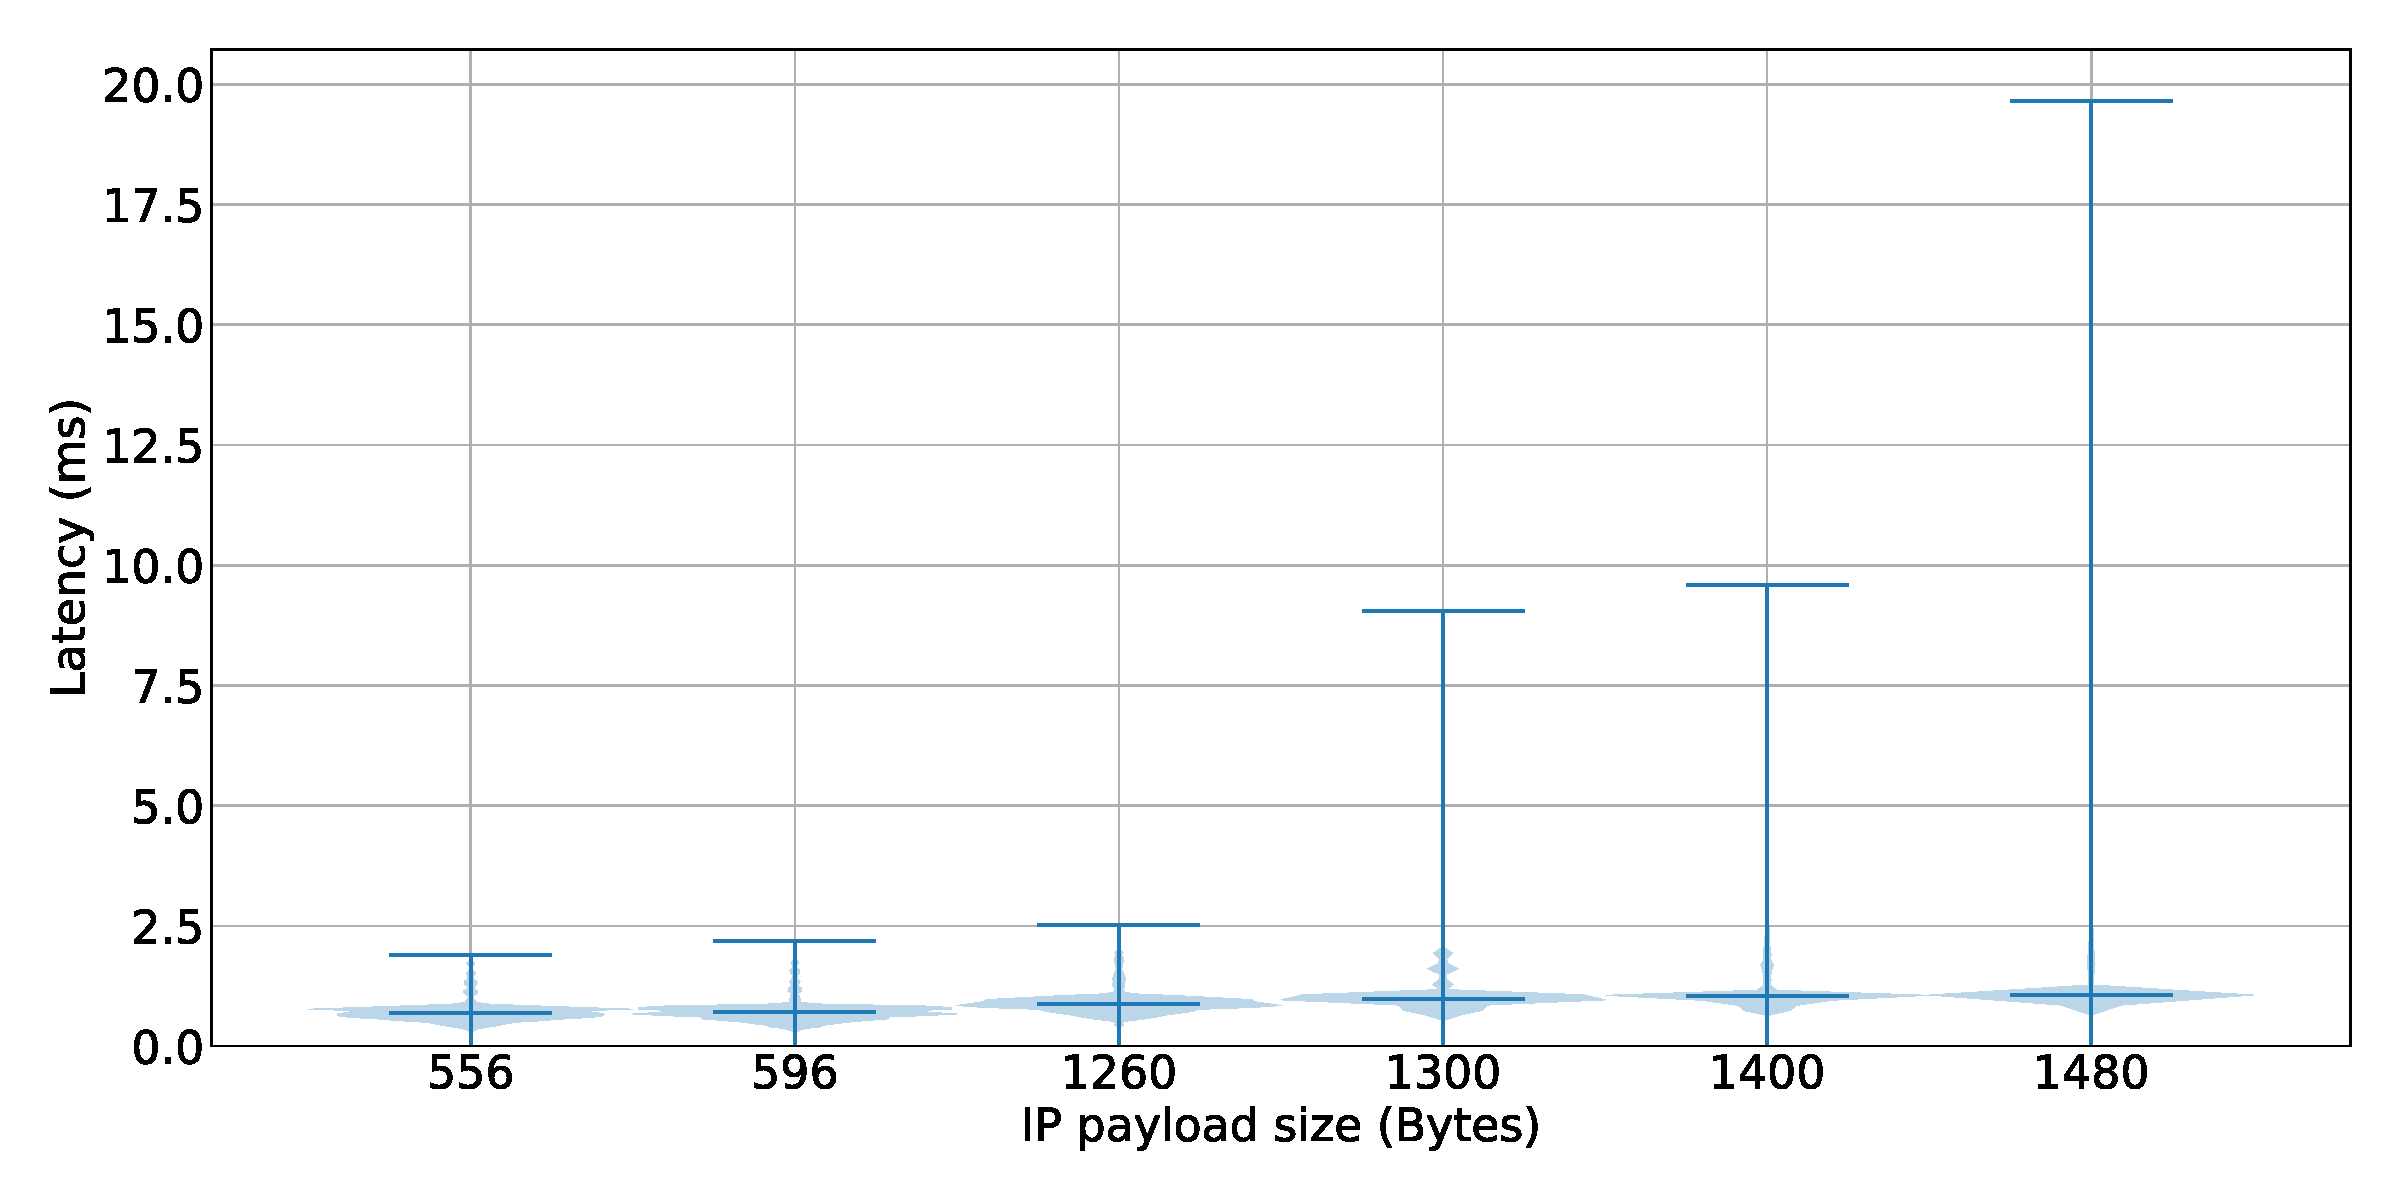
\includegraphics[draft=false,width=0.9\textwidth]{figures/Graphs/graph-1-mtu/latencies.pdf}
	\caption{Latencies for varying payload sizes}\label{fix:graph-1-mtu-latencies}
\end{figure}
Latency stays pretty much constant, with different packet sizes

only the tail latency is increasing drastically, which is unexpected.

\begin{figure}[tbh]
	\centering
	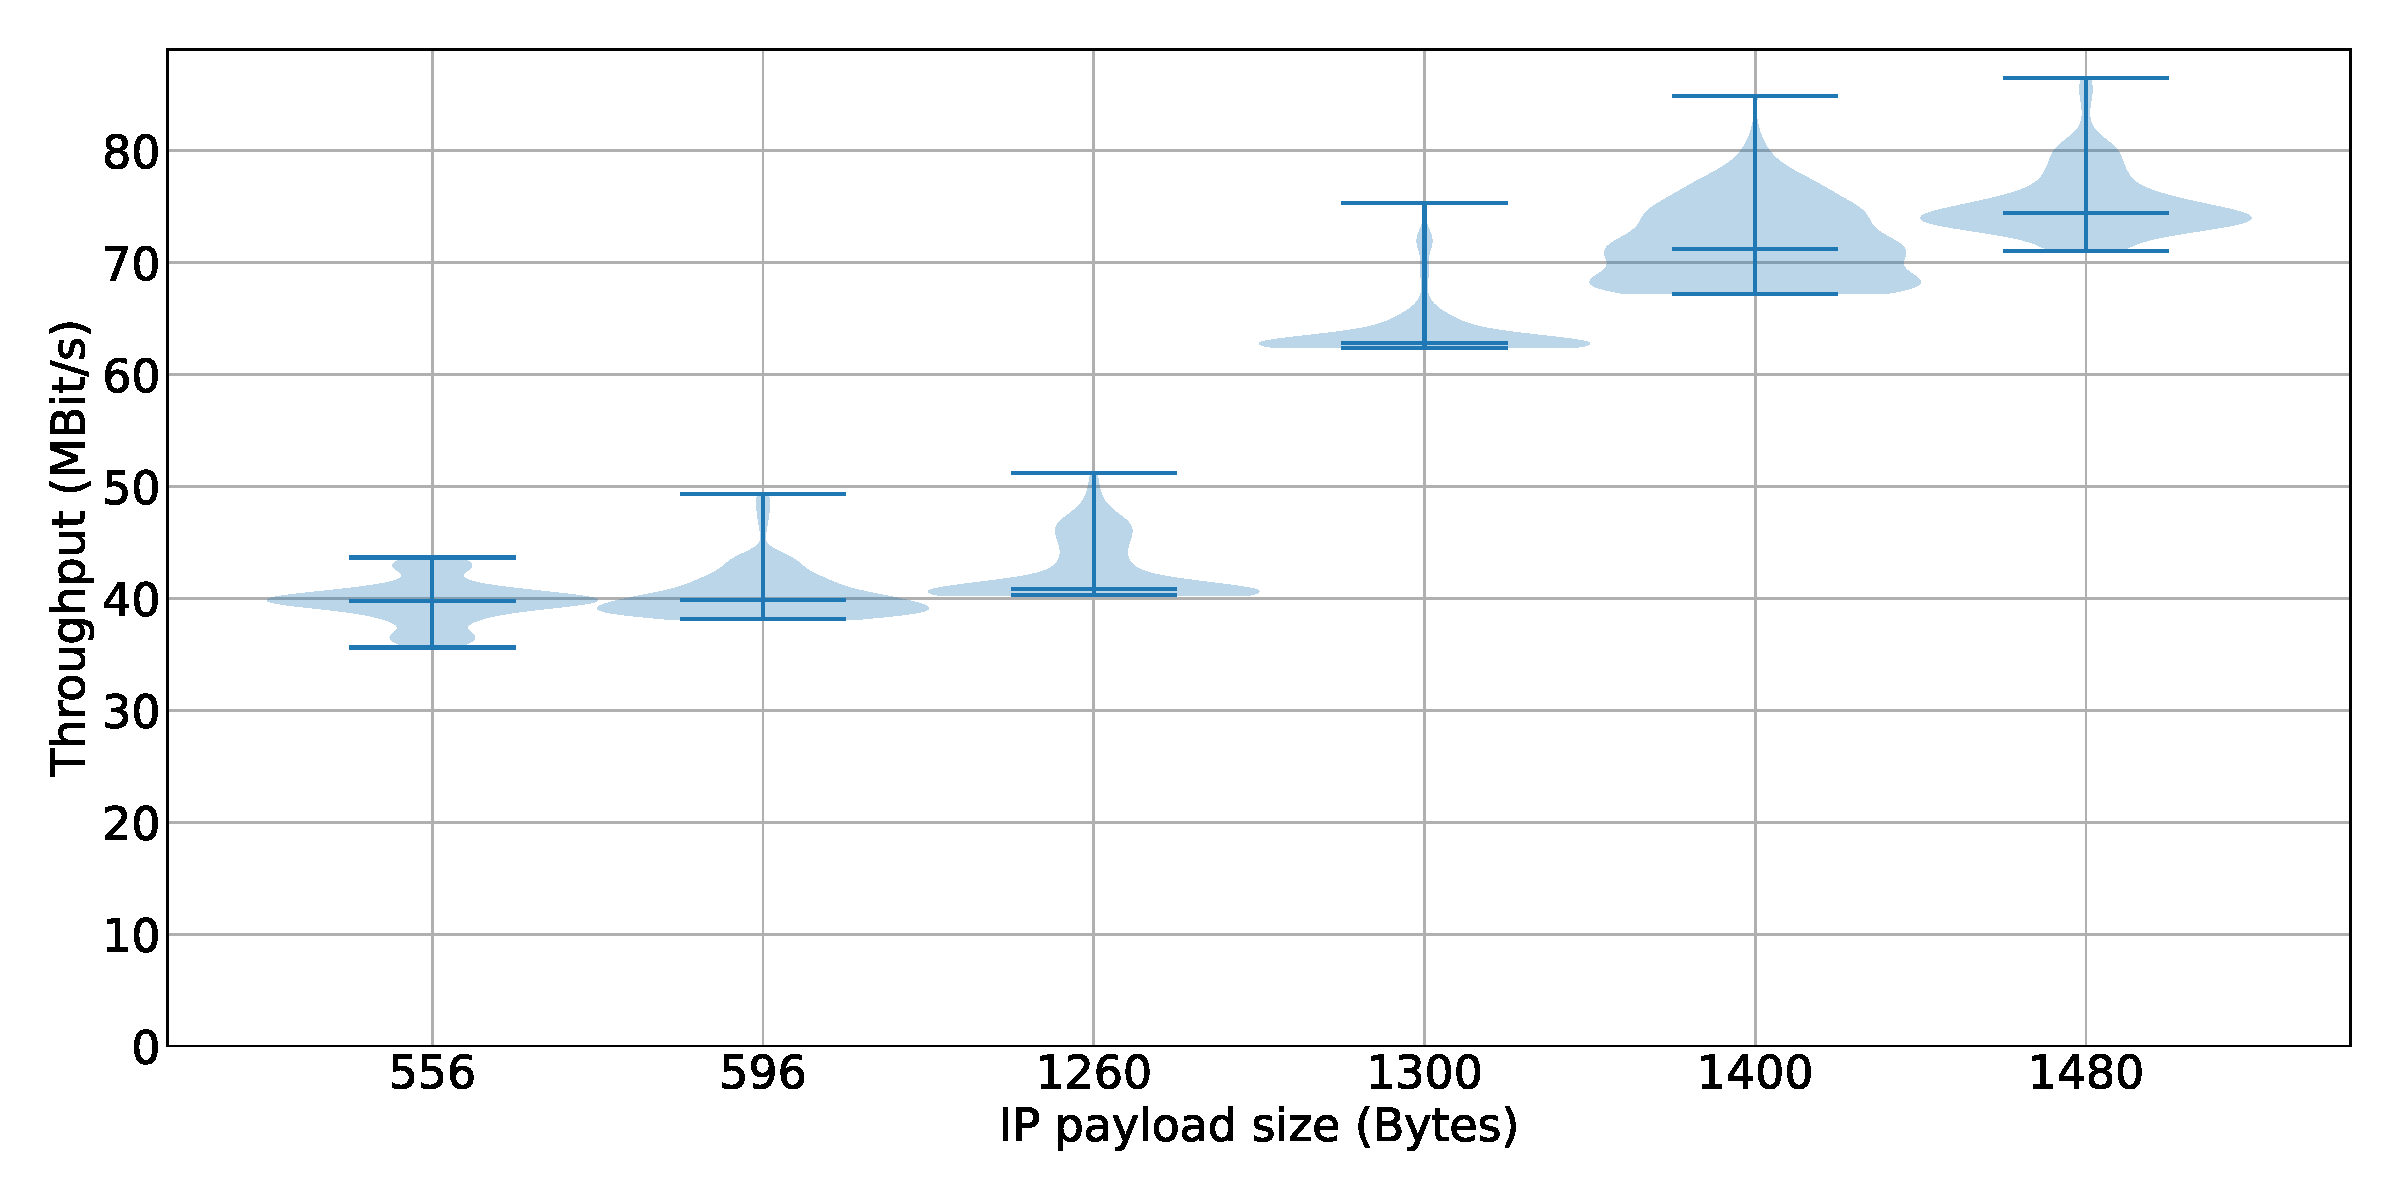
\includegraphics[draft=false,width=0.9\textwidth]{figures/Graphs/graph-1-mtu/throughput.pdf}
	\caption{Throughput for varying payload sizes}\label{fix:graph-1-mtu-throughput}
\end{figure}

The different measurements are always plotted on the x axis.

latency: violin plot: measurement, latency

packet duplicate: violin plot: measurement, ratio duplicate to total sent

packet dropped: violin plot: measurement, ratio dropped to total sent

throughput (with and without overhead): violin plot: measurement, throughput


move to chapter methodology:
one second buckets


We were unable to evaluate ICMPTX.
The program has a bug, where it crashes almost immediately after iperf3 starts sending data through the tunnel.
It fails with the error message \texttt{sendto: No buffer space available}.
The issue was mentioned previously \cite{icmptx-sendto-no-buffer-space-avaiable}.
The maintainer proposed two workarounds but using either one alone or both at the same time did not resolve the issue.
The problem seems to occur when trying to send data into the tunnel at a faster rate than the underlying link can support.
Tunnel software should be able to handle this case by dropping packets instead of crashing.


iodine

only one packet can be in flight, so usable throughput depends on latency and is generally very low

seems to not be true, since observed data rate was higher than expected

perhaps only the case in one direction?

Can not be measured reliably with our setup, would need improved setup, see figure



mostly see what we expected

we measure exactly the latency, loss and duplication we told the network emulator to simulate

measured throughput is influenced by number of dropped packets


Tor pluggable transports like obfs4 and Snowflake
meant for stream data like TCP, not UDP
\todo[inline]{Verify this claim more thouroughly!}

since we're only sending UDP packets, cannot be measured

would need a different test setup with a connection oriented data stream to test

instead of packet oriented

or some kind of UDP over TCP tunnel

this would also be influenced by congestion control algorithm


Rather than only a handful of combinations of parameters, as described in \cref{chap:methodology}, we tested many more.
In the beginning we even tested the cartesian product of all parameters.
This fact combined with several slightly different versions of our test setup, lead us to collect about 5 TB of packet captures, which compress to a little more than half of that using the zstd compression algorithm in Btrfs.

% SPDX-FileCopyrightText: 2024 Lukas Zirpel <thesis+lukas@zirpel.de>
% SPDX-License-Identifier: GPL-3.0-only

\chapter{Discussion}
\label{chap:discussion}
\todo[inline]{Forschungsfragen beantworten, bemerkenswerte Dinge aufschreiben}
Having presented the results of our experiments, this chapter delves into a comprehensive discussion of their meaning and implications.
We explore the impact of network impairments on protocol effectiveness and discuss the implications for the design of robust censorship evasion protocols.
Finally, we acknowledge the limitations of our study, outlining potential areas for improvement and future research.


\section{RQ1: How much packet size overhead does each protocol add?}
While we aimed to quantify the precise packet size overhead introduced by each protocol, our experimental setup did not allow for direct measurement of this metric.
However, it is important to note that the packet size overheads of many protocols are generally constant.
This overhead is due to the protocol’s header, which is added to the data payload.

When WireGuard is being transported over IPv4, its overhead breaks down as follows: The IPv4 header adds 20 bytes of overhead (when no IPv4 options are used), UDP another 8 bytes, and the WireGuard header itself 32 bytes, for a total of 60 bytes of overhead.

ICMPTX only supports ICMPv4, so its overhead consists of the IPv4 header (20 bytes) and the ICMP header (8 bytes) \cite{RFC0792} for a total of 28 bytes per packet.

Iodine's overhead is more complex and depends on the specific DNS record type, the direction of data transfer, and other factors, such as how many fragments iodine creates.
When it detects that the \texttt{NULL} record type is not filtered, it uses this type by default.
For IPv4 and sending data from the server to the client, the overhead breaks down as follows:
20 bytes for the IPv4 header, 8 bytes for the UDP header, 12 bytes for the DNS header, and a varying amout of overhead from iodine itself, depending depending on several factors as written above.
The exact overhead is not documented and reading the source code is required for gaining a detailed and accurate understanding of the overhead all combinations of packet sizes and DNS record types.
In our testing with IPv4 packets of 1130 bytes, the packet size outside of the tunnel increased to 1177 bytes, for a total overhead of $1177 - 1130 = 47$ bytes.



\section{RQ2: How much does the MTU decrease by using each protocol?}
For protocols that do not support fragmentation by themselves, the theoretical MTU decrease is directly related to the protocol's overhead.

We start with an MTU of 1500 bytes without any tunnel protocols.

When WireGuard is being transported over IPv4, its overhead is 60 bytes, as calculated above, so the maximum possible MTU without fragmenting any IP packets is $1500 - 60 = 1440$ bytes.
An IPv6 header (without extension headers) is 20 bytes larger than an IPv4 header, so if WireGuard is being transported over IPv6, the MTU is reduced to 1420 bytes.
This seems to be the default MTU systemd-networkd uses for WireGuard interfaces to allow it being transported over either IPv4 or IPv6 without changing the MTU.

The default MTU of ICMPTX is 1500 bytes because this is the default MTU of tun interfaces on Linux and ICMPTX neither changes the value by itself or tells the user to change it.
This choice will result in IPv4 packets being fragmented if packets are sent into the tunnel with a size larger than $1500 - 28 = 1472$ bytes.

iodine uses an MTU of 1130 bytes by default for its tunnel interface.
This is out of spec for transporting IPv6 packets:
\blockquote[\cite{RFC8200}]{IPv6 requires that every link in the Internet have an MTU of 1280 octets or greater.
This is known as the IPv6 minimum link MTU.
On any link that cannot convey a 1280-octet packet in one piece, link-specific fragmentation and reassembly must be provided at a layer below IPv6.}

It is possible to increase the MTU of the tunnel interface to above the path MTU outside of the tunnel minus the tunnel overhead.
In this case, the payload data combined with the tunnel overhead becomes too large to be transported over the network and the IP packet needs to be fragmented.
This results in less than optimal performance but may be desired in specific situations, such as when bridging layer 2 networks.


\section{RQ3: How much additional latency does each protocol add?}
Unfortunately, the measurement setup was not designed correctly to accurately capture the additional latency introduced by each protocol.
Measuring this requires observing the packets before they enter the tunnel and after they exit it.
The additional latency introduced by the protocol can then be analyzed by measuring how long each packet takes on average and subtracting the latency when no protocol is being used.
See \Cref{fig:optimal_network_schematic} for a setup, which would be up to the task.
While we acknowledge the importance of latency as a performance metric, we are unable to reliably quantify it within the constraints of our current experimental design.


\section{RQ4: Do any protocols introduce additional packet loss?}
Similarly to latency measurements, our setup is not equipped to reliably measure packet loss introduced by the protocols themselves.


\section{RQ5: How much processing power and RAM does each protocol consume/require?}
Our observations indicate that WireGuard's CPU usage remains mostly constant over time but is surprisingly not consistent across both sides of the tunnel.
During our tests, WireGuard consumed approximately 4\% on the sending side (server) and 10\% CPU on the receiving side (client).

We were unable to measure the CPU utilization of ICMPTX due to it crashing.
It used up to 2.3 MB of memory before doing so, both on the client and the server.

iodine used 100\% of the CPU on the sending side and 35\% on the receiving side, while the highest observed RAM usage was 1.7 MB on both sides.


\section{Limitations}
In reflecting on our work, we identify several areas where improvements could be made.

First and foremost, we recognize a fatal flaw in our measurement methodology.
The following scenario illustrates this flaw well:\\
Let's suppose we are testing a fictitious tunnel protocol, which splits all packets sent into the tunnel into two fragments, wraps them in its own header, and sends them onwards separately.
The protocol does not implement its own retransmission mechanism.
Only when both halves reach the other side of the tunnel can the original packet be reassembled.
If every second packet gets lost, then no packet can ever be reassembled at the receiver.
But our setup cannot measure this behavior since we only record packets when they are wrapped in the tunnel protocol and before they are unpacked and reassembled.
Our setup measures a packet loss of 50\%, while 100\% is the correct value.
The throughput is similarly measured incorrectly.
\Cref{fig:optimal_network_schematic} shows an improved setup capable of correctly measuring this behavior.
It allows recording the packets also before they enter the tunnel and after they exit it.

In particular, this allows us to properly evaluate the overhead of iodine, which depends on the particular DNS record type the program chooses at runtime.

Early on, we evaluated the Cartesian product of all parameters, which leads to an explosion of different combinations, which take a long time to measure.
We did this before deciding how to analyze and compare these many different combinations.
To mitigate this, we focus on isolating variables during testing—keeping all parameters constant except for the one being measured—to create meaningful graphs and reduce the number of required tests drastically.

Additionally, while we use iperf3 for our measurements, its requirement for both an initial UDP handshake and a TCP control connection brings several problems.
iperf3 fails to start the measurement when a critical UDP packet is lost and does not attempt to re-send it.
A pull request to improve this situation in iperf3 has existed for several years but it has not been merged yet \cite{iperf-udp-connect-retry}.
For our testing we apply this patch to make connection establishment reliable.
The initial handshake may also delay the start of the test, especially under high latency and high loss conditions.
In addition to that, the persistent TCP connection adds a very small amount of extra traffic, which is not under our control.
For our purposes it would be better to use a different traffic generator, which just sends random UDP packets, without any connection setup or control connection.

Another limitation is that we only use IPv4 since we need a common baseline but not all protocols support transporting IPv6 (iodine in particular).
We need to address this gap to ensure comprehensive evaluation across different network configurations.

Furthermore, we only transfer data in one direction and do not test protocols in both directions for ensuring their behavior is symmetric.
This is especially relevant for iodine, where we know with certainty that its bandwidth is asymmetric.

The packet queue in the router is not large enough, leading to dropped packets when trying to introduce a delay of 200 ms or longer.
Increasing the buffer size would resolve this limitation.

The router in our setup is connected to a 100Mbit/s port of the switch using a single Ethernet cable and two VLANs.
Both the client and the server are theoretically able to send and receive at full speed at the same time (each device 200Mbit/s in total) thanks to full-duplex.
But the router is effectively limited to half-duplex speeds as it has to send all data it receives back over the same link.
This presents an unintended bottleneck if data flows in both directions at the client and server at a fast enough rate.
While we attempt to avoid this situation by telling iperf3 to only send data in one direction, a small amount of data is still exchanged in both directions by iperf3's control connection, by our own control connection coordinating the test and by background noise like ARP messages.
To solve this limitation, the router could either be connected to a 1Gbit/s port of the switch or we could use two physical cables and interfaces instead of two VLANs.

We also did not test the influence of reducing the maximum bandwidth in the router.

Furthermore, preventing state from previous tests from influencing future ones is important.
While we acknowledge that one of the most reliable ways of achieving this goal is to restart all systems between tests, we don't do this due to time constraints and the added complexity of rebooting all hosts and waiting for them to be reachable, fully booted, and settled.
Netbooting all hosts goes one step further as without persistent storage, there are very few places left for state to accumulate.

Some unit tests for our data analysis scripts would have been nice to have and would have likely found at least one particular bug.

Finally, while modifying the NixOS test driver to scale to thousands of tests without running out of memory and with an evaluation time proportional to the number of protocols instead of the number of tests, we copy some parts of the driver from Nixpkgs.
We did however not copy the code that allows controlling the test interactively, which would have enhanced debuggability by not requiring a full rerun of the test after each change.
Addressing this limitation should be relatively simple.
\todo[inline]{try to write a couple more sentences so this sentence is not alone on a page}


%%% Local Variables:
%%% TeX-master: "thesis"
%%% End:

% SPDX-FileCopyrightText: 2024 Lukas Zirpel <thesis+lukas@zirpel.de>
% SPDX-License-Identifier: GPL-3.0-only

\chapter{Conclusion}
\label{chap:conclusion}

\todo{kurz und bündig Forschungsfragen beantworten}
We measured the performance of several different censorship circumvention protocols and compared them. Some behaved very well in less than ideal network conditions, others not so much.

\section{Future Work}

\appendix

\addtocontents{toc}{\vspace{5mm}}

% SPDX-FileCopyrightText: 2024 Lukas Zirpel <thesis+lukas@zirpel.de>
% SPDX-License-Identifier: GPL-3.0-only

\chapter{Appendix}
\label{chap:appendix}

Things upstreamed to Nixpkgs for this Thesis:
\begin{itemize}
  \item \href{https://github.com/NixOS/nixpkgs/pull/343277}{blake3 Python library (BLAKE3 cryptographic hash function)}
  \item \href{https://github.com/NixOS/nixpkgs/pull/360435}{Update blake3 Python library}
  \item \href{https://github.com/NixOS/nixpkgs/pull/281636}{Update the reuse tool}
  \item \href{https://github.com/NixOS/nixpkgs/pull/333462}{Allow easily changing the iperf3 package}
  \item \href{https://github.com/NixOS/nixpkgs/pull/357574}{ICMPTX program} (not yet merged)
  \item \href{https://github.com/NixOS/nixpkgs/pull/326845}{U-Boot for Orange Pi Zero3}
  \item \href{https://github.com/NixOS/nixpkgs/pull/362173}{Allow using ghostscript in a reproducible way, required for reproducible generation of this PDF document}
\end{itemize}


\renewcommand{\emph}{\textit}

\printbibliography

\end{document}

%%% Local Variables:
%%% mode: latex
%%% TeX-master: t
%%% End:
